\documentclass[12pt]{article}
\usepackage{amsfonts, epsfig}
\usepackage[authoryear]{natbib}
\usepackage{array}
\usepackage{multirow}
\usepackage{graphicx}
\usepackage{fancyhdr}
\usepackage{amsmath}
\usepackage{amssymb}
\pagestyle{fancy}
\lfoot{\texttt{semtm0051.github.io} }
\lhead{Autoencoder - Conor}
\rhead{\thepage}
\cfoot{}

\usepackage{tikz}
\usetikzlibrary{positioning}
\usetikzlibrary{decorations.pathreplacing, calc}

\usepackage{ifthen}
\newboolean{nopics}
\setboolean{nopics}{true}


\begin{document}

\section*{Autoencoder} 

The work ``auto'' generally means ``self'' and an autoencoder is a
network that returns something close to the same output as it used for
input. This might seem like an odd thing to want to do but we are
going to look at autoencoders for two reasons, the first is that they
do have a use, an autoencoder with a bottleneck, a intermediate layer
that is smaller than in the input, is useful since it forces the
network to summarize the input if it wants to still be able to
reproduce the output. You still see auto-encoders used in this way and
this use of an auto-encoder is similar to some approaches, like
word2vec, that are interesting to consider. Another class of
autoencoders, the sparse autoencoder, has become a useful tool for
examining the behaviour of large transformers. We will learn about
sparse autoencoders in the workshop. However, we are really more
interested in the second reason, that the autoencoder demonstrates one
aspect of what is happening inside a more general network, networks
work through a series or representations and encodings and we can use
a simple autoencoder to see that happening.

\begin{figure}
  \centering
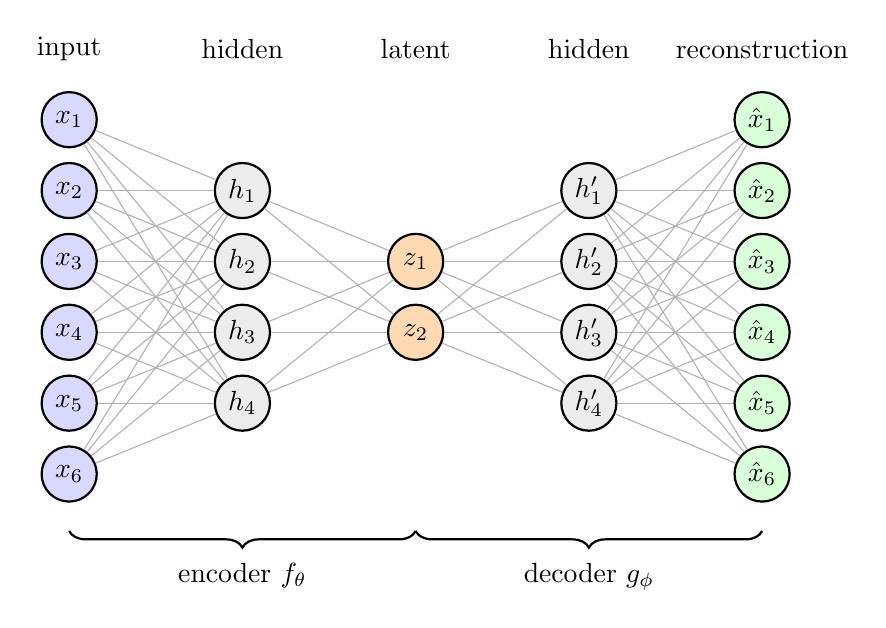
\begin{tikzpicture}[
    x=2.2cm, y=0.9cm,
    neuron/.style={circle, draw, thick, minimum size=7mm, inner sep=0pt},
    inp/.style={neuron, fill=blue!15},
    hid/.style={neuron, fill=gray!15},
    code/.style={neuron, fill=orange!30},
    outp/.style={neuron, fill=green!15},
    conn/.style={-, gray!60, line width=0.4pt},
    brace/.style={decorate, decoration={brace, amplitude=6pt}, thick}
  ]

  % --- sizes: change these to resize the network ---
  \def\nin{6}   % input / output width
  \def\nhid{4}  % hidden width
  \def\ncode{2} % bottleneck width

  % input layer
  \foreach \i in {1,...,\nin}
    \node[inp] (x\i) at (0, {(\nin+1)/2 - \i}) {$x_{\i}$};

  % encoder hidden layer
  \foreach \k in {1,...,\nhid}
    \node[hid] (h\k) at (1, {(\nhid+1)/2 - \k}) {$h_{\k}$};

  % bottleneck (code) layer
  \foreach \j in {1,...,\ncode}
    \node[code] (z\j) at (2, {(\ncode+1)/2 - \j}) {$z_{\j}$};

  % decoder hidden layer
  \foreach \k in {1,...,\nhid}
    \node[hid] (g\k) at (3, {(\nhid+1)/2 - \k}) {$h'_{\k}$};

  % output layer
  \foreach \i in {1,...,\nin}
    \node[outp] (y\i) at (4, {(\nin+1)/2 - \i}) {$\hat{x}_{\i}$};

  % connections
  \foreach \i in {1,...,\nin}
    \foreach \k in {1,...,\nhid} {
      \draw[conn] (x\i) -- (h\k);
      \draw[conn] (g\k) -- (y\i);
    }
  \foreach \k in {1,...,\nhid}
    \foreach \j in {1,...,\ncode} {
      \draw[conn] (h\k) -- (z\j);
      \draw[conn] (z\j) -- (g\k);
    }

  % layer labels (all at a common height)
  \foreach \pos/\lab in {0/input, 1/hidden, 2/latent, 3/hidden, 4/reconstruction}
    \node at (\pos, {(\nin+1)/2}) {\lab};

  % encoder / decoder braces
  \draw[brace, decoration={mirror}]
    ($(x\nin.south)+(0,-0.4)$) -- ($(z\ncode.south |- x\nin.south)+(0,-0.4)$)
    node[midway, below=8pt] {encoder $f_\theta$};
  \draw[brace, decoration={mirror}]
    ($(z\ncode.south |- y\nin.south)+(0,-0.4)$) -- ($(y\nin.south)+(0,-0.4)$)
    node[midway, below=8pt] {decoder $g_\phi$};

\end{tikzpicture}
\caption{A schematic of an autoencoder; the input $\mathbf{x}$ comes
  in on the left and gets mapped to a putative output
  $\mathbf{\hat{x}}$ on the right. The network is trained by
  minimizing an error function that measures the different between
  $\mathbf{x}$ and $\mathbf{\hat{x}}$; the obvious error is just
  $|\mathbf{\hat{x}}-\mathbf{x}\|^2$ but it isn't always the error
  used. Here, of course, the hidden layers might refer to more than
  one layer but often the idea of having the middle layer smaller than
  in the input is common, this middle layer is often called the latent
  space.\label{fig:ae}}
\end{figure}


A schematic for an autoencoder is shown in Fig.~\ref{fig:ae} and an even more succint summary would be:
\begin{equation}
\text{original}\rightarrow \text{hidden}\rightarrow \text{latent} \rightarrow \text{hidden}\rightarrow\text{reconstruction}
\end{equation}
and for now we are imaginging that the latent space is smaller than
the original, so it should find the representation of the original
data that represents the important part of the signal allowing it to
be broadly reconstructed, in general. We have seen before how this
might work, in PCA for many classes of data the first few principle
components contain most of what is important in the signal. Indeed,
autoencoders can be thought of as a non-linear version of principle
component analysis
\footnote{You could argue that, in principle, no summarization needs
to take place, since a continuous number has infinite capacity to
store information, reducing the number of dimension need not mean
disgarding information. However, what neural network learning learns
tends not to exploit things like that; thanksfully, the effectiveness
of deep learning, its ability to generalize, relies in part on it not
performing that sort of annoying trick.}.

The best thing is to look at an example and before doing that it is
useful to introduce MNIST; MNIST is the `hello world' dataset for
images and neural networks. It is a set fof 60,000 training images and
10,000 test images. Each is a 28$\times$28 greyscale grid showing a
digit from zero to nine; the original data was binary, black and
white, but anti-aliasing at some point introduced greys, in practice
the pixels are mostly white or near white, or black or near black.

The US National Institute of Standards and Technology was asked by the
US census bureau to see if computers could be used to read handwritten
census forms, this lead to them collecting a set of handwritten
characters.  For MNIST the source is two NIST collection, segmented
from scanned Handwriting Sample Forms and stored as binary images:
Special Database 3, written by Census Bureau employees, and Special
Database 1, written by high-school students. For their paper
"Gradient-based learning applied to document recognition", LeCun,
Bottou, Bengio and Haffner used these datasets to make a new dataset
with a standard size, this became MNIST, the `M' is for modified. NIST
originally intended SD-3 for training and SD-1 for testing, but SD-3
is much cleaner and easier, so MNIST mixes them: 30,000 from each for
training and 5,000 from each for test, with SD-1's roughly 500 writers
split so that none appears in both sets.

Anyway the key point is that it is a standard dataset used as a first
test for image networks; it is an easy dataset to download and to load
into your programme, there are standard loaders and functions for
printing out images or reconstructions. There are also other datasets
that fit the same pattern that can be easily slotted in to a programme
that has been written for MNIST, the most famous is probably
fashionMNIST, the same size images, ten categories as before, but they
are outlines of ``fashion items'', shoes and bags and so on. The thing
is that fashionMNIST is harder for a network to classify than
MNIST. This points out a problem with MNIST, it is too easy, a linear
classifier can get the right answew 92\% of the time, a good
multi-layer network 98\% and a convolutional network 99\%; the
remaining digits are weird and indiosyncratic. This means as a dataset
it isn't a useful test of how good your network is, but it is a way to
check it is working. Some MNIST images are showning in Fig.~\ref{fig:mnist}.

\begin{figure}
\begin{center}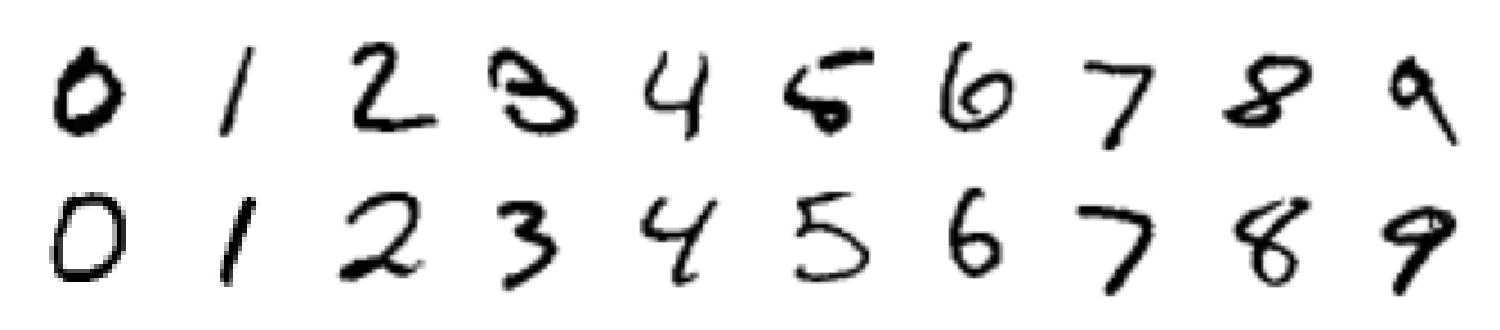
\includegraphics[width=0.95\textwidth]{mnist_samples.pdf}\end{center}
\caption{A few examples of MNIST images, there are 70,000 in total, 7,000 for each of ten digits.\label{fig:mnist}}
\end{figure}


So in our implementation\footnote{The code can be found in the \texttt{Slide} folder.} we use a 
\begin{equation}
784 \rightarrow 512 \rightarrow 256 \rightarrow 2 \rightarrow 256 \rightarrow 512 \rightarrow 784
\end{equation}
The latent layer is only two-dimensional and this isn't something
chosen for any better reason than that we want to plot it; if the
representations were being used for something else a larger latent
layer might be used. You might wonder what we'd be doing that would
use the latent layer, here is any example, imagine that we had a
larger collection of digits, but only a small fraction were
classified, but like MNIST but for most image the data didn't tell us
what digit the image represented. In this situation we can imagine
trying to set up a combined workflow with unsupervised and supervised
aspects. In the unsupervised part we would run the data through an
autoencoder, this would extract the `shape' of the data, what's
happening in the image; this is encoded in the latent representation,
the activity of the latent layer. For the subset of images with labels
we would then run a classifier on the latent representations,
typically this gives much better results than running the classifier
on the original images.

Anyway back to our actual example where we are auto-encoding MNIST; in
this case we aren't trying to classify, we are just looking at what
the latent representations show us. To give a few details the hidden
layers all use ReLu: $\phi(u)=\max(0,u)$ except the latent space, this
is linear, so $\mathbf{z}\in\mathbb{R}^2$. We use a sigmoid for the
output so $\hat{x}_i\in[0,1]$. The loss is binary cross-entropy loss:
\begin{equation}
  L=-\sum_{i=1}^{784}\left[x_i\log\hat{x}_i+(1-x_i)\log(1-\hat{x}_i)\right].
\end{equation}
Of course, this is one of the two obvious loss functions, the other is
the $L^2$ error, as noted above. Why cross-entropy rather than $L^2$?
Well either would be fine, and neither has particular theoretical
support. From an engineering point-of-view, given that the true values
of the pixels saturate, they are either zero or one, mostly, and the
sigmoid is flat there, the $L^2$ gives low gradients in that region.

\begin{figure}
\begin{center}
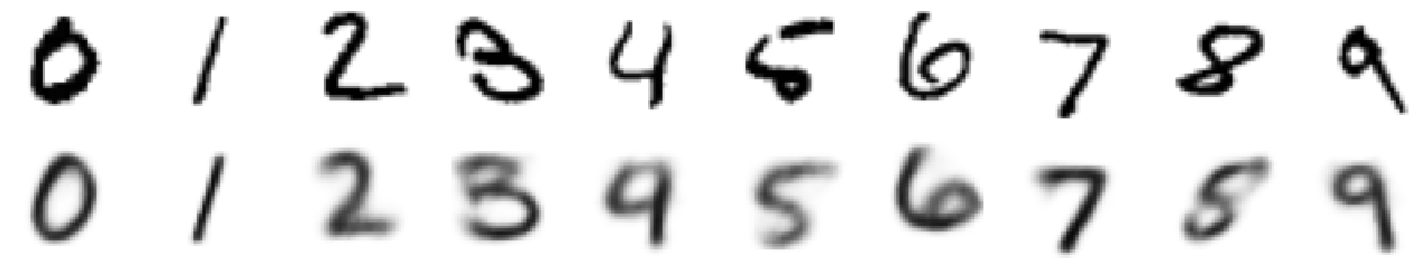
\includegraphics[width=0.95\textwidth]{reconstructions.pdf}
\end{center}
\caption{The reconstruction for a random example for each digit, the original on top, the reconstruction below. It is clear that the image hasn't come through unscathed; a bit of blurring you might expect, but the four and the eight are pretty bad. Clearly this depth of network struggles to fit everything into two-dimensions.\label{fig:recon}}
\end{figure}


\begin{figure}
\begin{center}
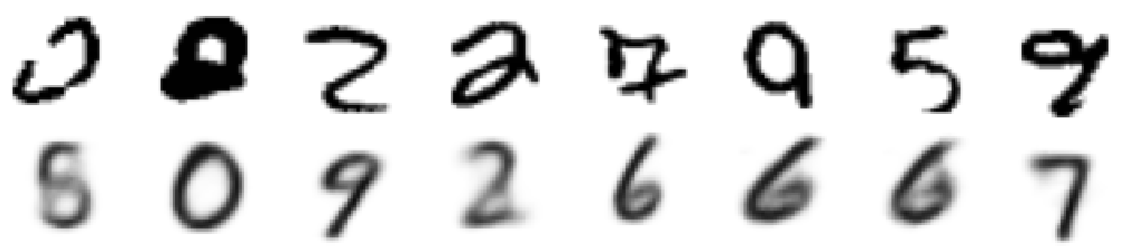
\includegraphics[width=0.8\textwidth]{worst_reconstructions.pdf}
\end{center}
\caption{The reconstruction for some of the worst examples, the original on top, the reconstruction below. Obviously the originals have odd features that don't occur often in the data set, the thick blob in 454 for example, these features aren't ones that the two dimensional latent space encodes.\label{fig:worst}}
\end{figure}

\begin{figure}
\begin{center}
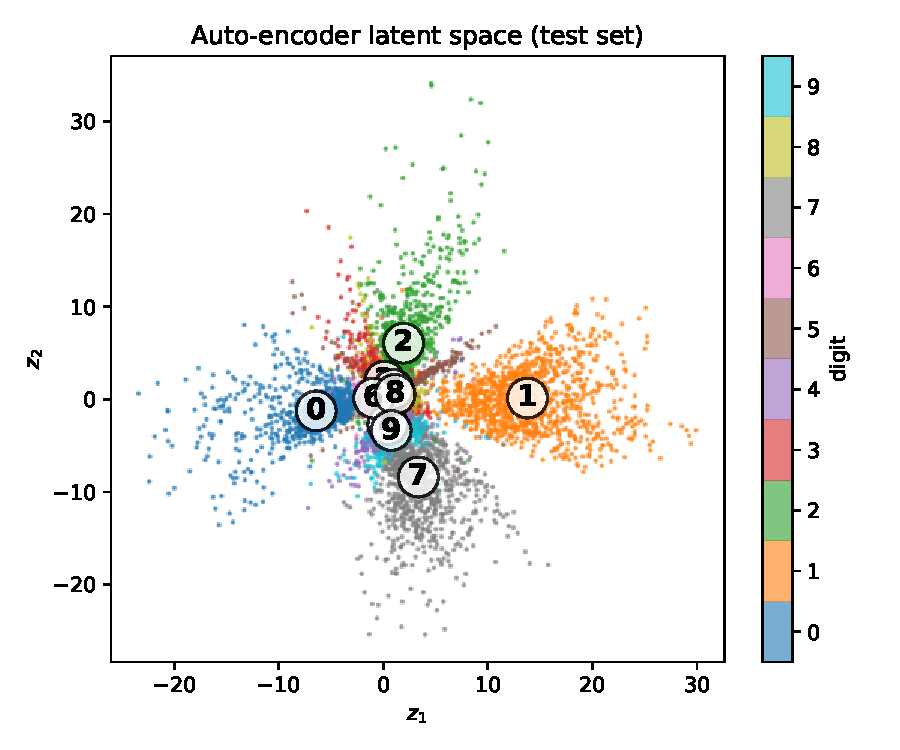
\includegraphics[width=\textwidth,height=0.82\textheight,keepaspectratio]{latent_scatter.pdf}
\end{center}
\caption{A random subset of the data points mapped to the latent space
  and coloured by their label. The ones, sevens, zeros, twos and to a
  certain extend threes have features that seperate them, the rest end
  up in a blob in the middle.\label{fig:latent}}
\end{figure}

The results of the reconstructions are showing in
Fig.~\ref{fig:recon}; we can see the network does reconstruct the
digits digits through it clearly struggles a bit with some digits. In
Fig.~\ref{fig:worst} we see the worst reconstructions, here we can see
it has had some unusual input and has clearly sent it to the `wrong
place' in the latent space so when it is reconstructed it looks
completely wrong. Anyway the intesting thing is to look at the way the
data has been arranged in the latent space. In Fig.~\ref{fig:latent}
we see the points coloured by their digit, but remembering that this
is an autoencoder, the learning is unsupervised, so the labelling in
the figure is to illustrate what the latent space looks like. We can
see the features it find and represents, the ones with their straight
line to the right, the round zeros to the left, sevens with the cross
bar below, the two above.


\begin{figure}
\begin{center}
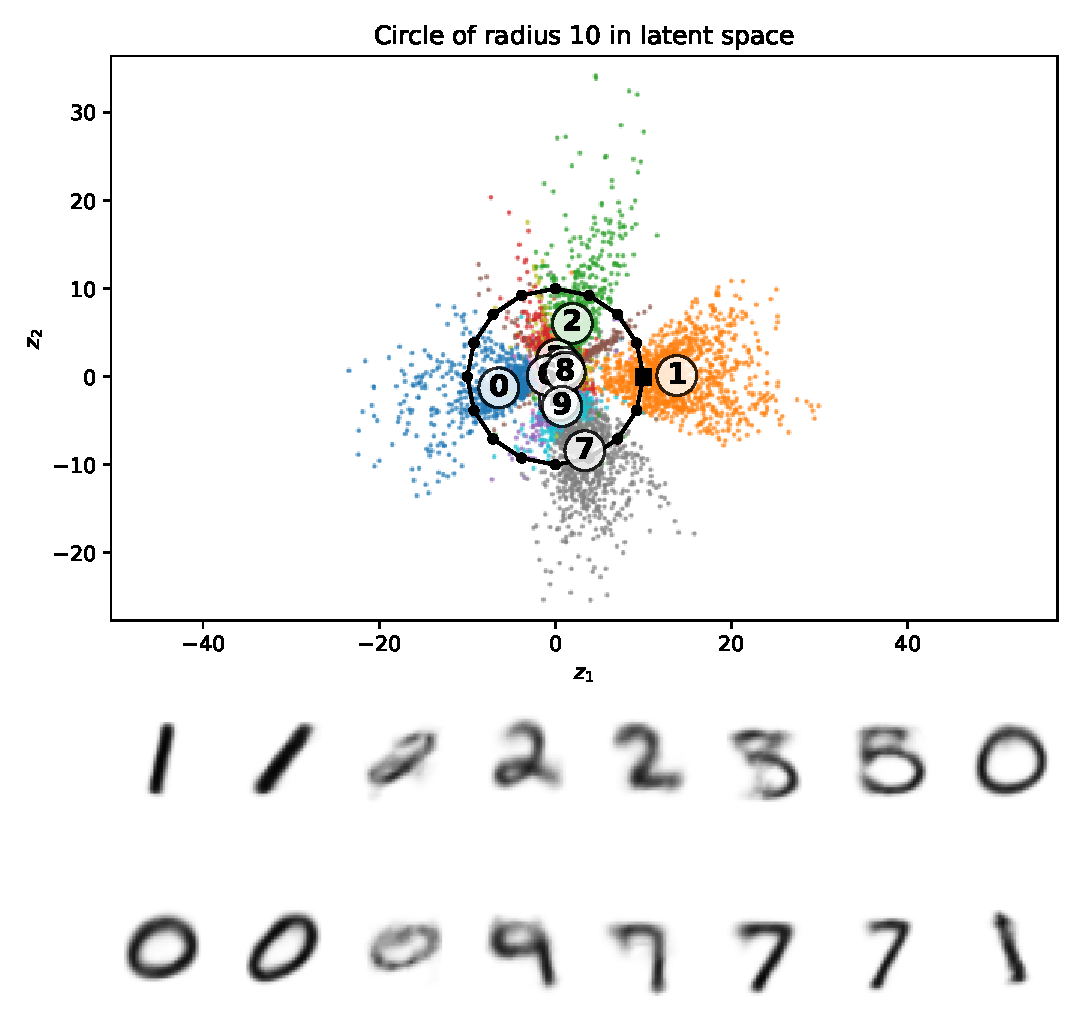
\includegraphics[width=\textwidth,height=0.82\textheight,keepaspectratio]{latent_circle.pdf}
\end{center}
\caption{A circle through the latent space. Here 16 points from a circle of radius ten are reconstructed, showing how one figure morphs into another as you move around the circle.\label{fig:circle}}
\end{figure}

\begin{figure}
\begin{center}
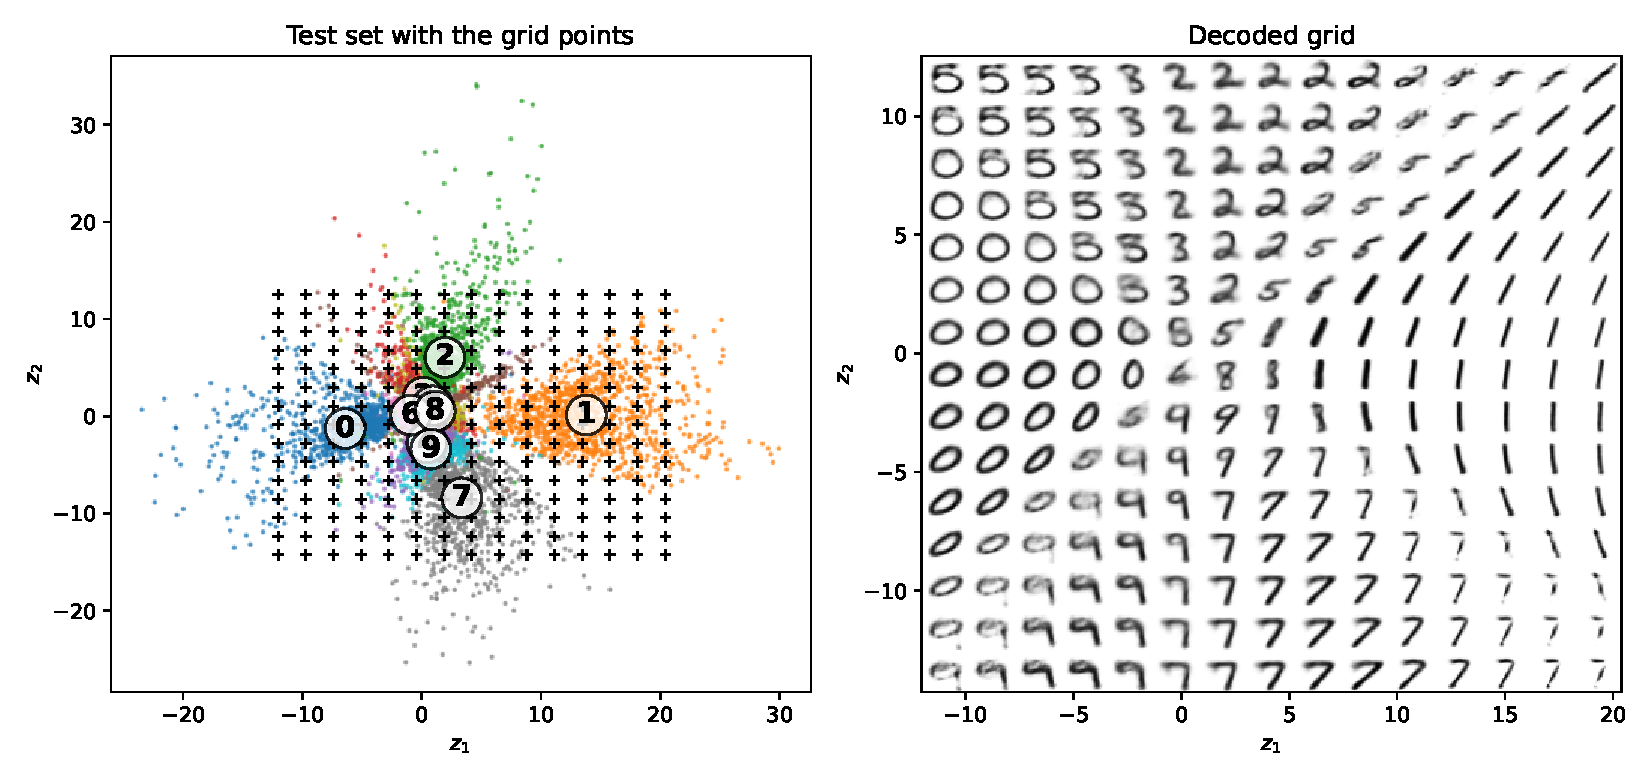
\includegraphics[width=\textwidth,height=0.82\textheight,keepaspectratio]{latent_grid.pdf}
\end{center}
\caption{A grid of points. Here a grid of points in the latent space are reconstructed, we can see the shapes changes from one digit to another, but not in a way that 'sticks' to the space of plausible digits.\label{fig:grid}}
\end{figure}

Fig.~\ref{fig:circle} gives us a better idea of what is working and
what is not working in the latent representation; overall the message
of this lecture is that networks compute using a series of
representations and the latent representations of the autoencoder are
being used to illustrate this. Here we see that the latent
representation is doing something useful, it is arrange the
two-dimensional space so that different features appear in different
areas and as we go around the circle in Fig.~\ref{fig:circle} we see
them appearing and disappearing. However, we also see that the latent
representations `understanding' of the features is not very
`feature-ey'. It is not moving around lines, bending edges as it goes
from one area to another, it is fading pixels in and out. In other
words, in this simple network it is still dealing with pixels rather
than what we would think of as the features, the edges. To go from a
two to a three we might think about extending the bottom line and
curving it around or something, the latent representation is just
fading out the pixels at the bottom of the two and fading in the
pixels of the three. In otherwords, the latent representation is
making some sort of sensible organization of the features, two and
three share a curved upper edge and are beside each other, but it
doesn't have a high-level feature based understanding of what makes a
digit. This has a few lessons for us, the first is that the
autoencoder is organizing the digits in a sensible way but that this
small network isn't reaching a high-level feature-based representation
and, perhaps, the interesting thing is that it largely succeeds
without doing that.

The other interesting failure of the latent space is illustrated in
Fig.~\ref{fig:grid}; this goes further in looking at the
reconstructions over a grid in the latent space. We see that the
latent space doesn't represent the `space of plausible digits'. The
network hasn't found a two dimensional space of digits and mapped it
to the latent space, it has found a latent space which includes the
two-dimensional space of real digits: there are gaps, areas of the
latent space that don't map to genuine digits. This is a limitation,
we would like to understand the `space of digits' or to imagine that
our networks have an understanding of that space; this means
representing what is happening without gaps so that the morphing from
digit to digit happens through plausible digits. There is a
terminology for this; what we want is a \textsl{generative space}
rather than a latent space. Next we will look at \textsl{variational
  auto-encoders} as an approach to constructing generative spaces;
this is a very particular approach to constructing a network which
might look different from the elements of a transformer; a question
you might ask is whether there are aspects of how large networks are
trained or how they perform inference that make them behave more like
variational auto-encoders than ordinary auto-encoders.

Firstly, what is a generative space? A generative space is a model of
the space of the data. The idea is that you start with a space
$\mathcal{Z}$ that sort of corresponds to the fundamental causes of
what we see, this is mapped to what we do see $\mathcal{X}$ and an
interesting and useful thing to do is to recover $\mathcal{Z}$ from
$\mathcal{X}$. To give a sort of classical example, imagine that
household income determine childhood nutrition and ultimately weight
and height in later life, the generative space is the household income
and the observed space is the weight and height, the latter is easy to
measure, the former is what we are interested in. Slightly more
formally, a \textsl{generative model} is a probability distribution
over the data that we can sample from, so it can produce new examples
that look like the training data, so it is a random variable $Z$ over
$\mathcal{Z}$ with a known $p_Z(z)$ so that if we sample $z$ and map
$z\rightarrow x$ the $x$ will look like the data.

\subsection*{The variational autoencoder}

We will introduce the VAE first as a sort of `engineering solution'
and then briefly outline the idea that there is a more mathematically
transparent approach. The idea is that there are gaps in the latent
space, the latent space puts ones in one place and sevens in the other
and in between it makes images that don't look like digits. The VAE is
intended to stop that and the way it does that is by introducing noise.
\begin{equation}
  \text{original} \rightarrow \text{latent} \rightarrow \textcolor{red}{\text{latent + noise}} \rightarrow \text{reconstruction}
\end{equation}
Adding noise to the latent representation means nearby points must
decode to similar images, so the gaps get filled in, `stitching
together' the representation. This looks something like this:
\begin{equation}
 \mathbf{x} \rightarrow
\begin{array}{c}\boldsymbol{\mu}=f_\mu(\mathbf{x})\\ \boldsymbol{\sigma}=f_\sigma(\mathbf{x})\end{array}
\rightarrow
\textcolor{red}{z_i\sim\text{Normal}(\mu_i,\sigma_i)}
\rightarrow
\hat{\mathbf{x}}=g(\mathbf{z})
\end{equation}
so the original is mapping to a latent space of means values and a
space of variances and then, before being allowed to reconstruct the
image these are used to find the slightly random latent representation.

Now still talking from an engineering point of view, adding noise is
obviously going to make the reconstructions worse. If the objective
function is not adjusted the system is going to cheat by making the
noise small, either by making the $\sigma$s very small or by making
the $\mu$s very big, the autoencoder has all sorts of scalling
invariances it can exploit to make the noise `harmless'. The solution
is to add an extra term to the objective function that pushes the $\mu$s towards zero and the $\sigma$s towards one:
\begin{equation}
L=\text{reconstruction error}+\sum_i\mathrm{KL}\big(\text{Normal}(\mu_i,\sigma_i)\,\|\,\text{Normal}(0,1)\big)
\end{equation}
The extra bit is a KL-divergence, a Kullback-Leibler divergence, which
is a standard measure, taken from information theory, of the
difference between two probability distributions; it is zero when the
two distributions are the same and gets bigger the more they differ.
In general it involves an integral, but when both distributions are
normal the integral can be done and the answer has a simple form, so
the objective function is just
\begin{equation}
L=\text{reconstruction error}+\frac{1}{2}\sum_i\left(\mu_i^2+\sigma_i^2-\log{\sigma_i^2}-1\right)
\end{equation}
and you can see how it works: the $\mu_i^2$ penalises any $\mu_i$ that
strays from zero, and $\sigma_i^2-\log{\sigma_i^2}-1$ is zero at
$\sigma_i=1$ and positive everywhere else, growing if $\sigma_i$ gets
big and, because of the logarithm, growing without limit as $\sigma_i$
shrinks towards zero, which is exactly the cheat we wanted to rule out.

This is a bit of a technical detail, but an important one; as it is currently described the step:
\begin{equation}
  z_i\sim\text{Normal}(\mu_i,\sigma_i)
\end{equation}
looks like a big problem for machine learning since it interupts the
autograd based calculation of partial derivatives preventing the
calculation of the gradients, or, put another way, it obstructs the
back-propagation of the errors from the reconstructions to the inputs. The way around this is to do what is often called the \textsl{reparameterization trick}. This rewrites the random step as
\begin{equation}
  z_i=\mu_i+\sigma_i \zeta_i
\end{equation}
where
\begin{equation}
  \zeta_i\sim\text{Normal}(0,1)
\end{equation}
This is functionally equivalent and, of course, the autograd should
still ignore the bit were the random number is calculated, the
$\zeta_i$ bit, but the important stuff, the $\mu_i$ and the $\sigma_i$
is there in a form that is available for back-propagation.


There is a more formal approach to all of this! This starts with an explicit description of the process in terms of a latent variable:
\begin{equation}
  \textcolor{red}{z_i\sim\text{Normal}(0,1)} \rightarrow x_j\sim\text{Bernoulli}\big(g_j(\mathbf{z})\big)
\end{equation}
where $j$ runs from one to 784 and labels the pixels, $x_j$ is the
value of the $j$th pixel and $g_j(\mathbf{z})$ is the $j$th output of
the decoder. This is a story about how a digit is made, read from left
to right: first a point in the latent space is picked from a fixed and
very simple distribution, this is called the \textsl{prior},
$p(\mathbf{z})$, and then the decoder turns that point into a
probability for each pixel being on, which gives the
\textsl{likelihood}, $p(\mathbf{x}|\mathbf{z})$; we are pretending
here that pixels are either on or off, which, as we saw, is nearly
true for MNIST. It is as if $\mathbf{z}$ is the idea of the digit and
the image is that idea in `disguise'. Notice that this is a generative
model in exactly the sense described above: there is a known
distribution on $\mathcal{Z}$, we can sample from it, and if the
decoder is any good what comes out the other end will look like the
data.

The decoder, then, goes from the idea to the image; the encoder has to
go the other way: given a digit $\mathbf{x}$, which $\mathbf{z}$
produced it? Since the story is a random one the answer is not a
single point, it is a distribution over $\mathbf{z}$, the
\textsl{posterior}, and Bayes' rule tells us what it is:
\begin{equation}
  p(\mathbf{z}|\mathbf{x})=\frac{p(\mathbf{x}|\mathbf{z})\,p(\mathbf{z})}{p(\mathbf{x})}
\end{equation}
The trouble is the denominator,
\begin{equation}
  p(\mathbf{x})=\int p(\mathbf{x}|\mathbf{z})\,p(\mathbf{z})\,d\mathbf{z}
\end{equation}
which requires running the decoder at every point of the latent space;
with only two latent dimensions you could just about do that on a
grid, but for a latent space of any useful size it is hopeless, the
integral is \textsl{intractable}. So we do not calculate the
posterior, we approximate it, and here we follow the general
philosophy of deep learning: if there is a function we need and do not
know, we make a network for it and learn it. The approximate posterior
is
\begin{equation}
  q(\mathbf{z}|\mathbf{x}):\quad z_i\sim\text{Normal}(\mu_i,\sigma_i),\qquad \boldsymbol{\mu}=f_\mu(\mathbf{x}),\quad \boldsymbol{\sigma}=f_\sigma(\mathbf{x})
\end{equation}
which is, of course, exactly the encoder we had before, the one we
arrived at by adding noise to stitch the latent space together; what
has changed is what we think it is for. This is sometimes called
\textsl{amortized} inference: rather than working out an approximate
posterior separately for each image, which is what you would do in
ordinary Bayesian inference, a single network is trained to give the
approximate posterior for every $\mathbf{x}$, so the cost of doing the
inference is spread over the whole dataset.

Now we need an objective function, and from this point of view there
is an obvious thing to want: the model assigns a probability
$p(\mathbf{x})$ to every possible image and we would like it to assign
a high probability to the images that are actually in the training
data, so we want to maximize $\log p(\mathbf{x})$ over the training
set. This is maximum likelihood, it is what fits the distribution of
the model to the distribution of the data. Of course $p(\mathbf{x})$
is precisely the thing we have just said we cannot calculate, but it
turns out we can get at it indirectly. From the definition of
conditional probability
\begin{equation}
  \log p(\mathbf{x})=\log p(\mathbf{x},\mathbf{z})-\log p(\mathbf{z}|\mathbf{x})
\end{equation}
and this is true for any $\mathbf{z}$; the left hand side does not
depend on $\mathbf{z}$ at all, so we can average both sides over
$\mathbf{z}$ drawn from $q(\mathbf{z}|\mathbf{x})$ without changing
it, and if we also add and subtract $\log q(\mathbf{z}|\mathbf{x})$
inside the average we get
\begin{equation}
  \log p(\mathbf{x})
  =\mathbb{E}_q\left[\log\frac{p(\mathbf{x},\mathbf{z})}{q(\mathbf{z}|\mathbf{x})}\right]
  +\mathbb{E}_q\left[\log\frac{q(\mathbf{z}|\mathbf{x})}{p(\mathbf{z}|\mathbf{x})}\right]
\end{equation}
The second term is, by definition, the KL-divergence between the
approximate posterior and the true one. In the first term we write
$p(\mathbf{x},\mathbf{z})=p(\mathbf{x}|\mathbf{z})\,p(\mathbf{z})$ and
split the logarithm, and this gives another KL-divergence, this time
between the approximate posterior and the prior:
\begin{equation}
  \log p(\mathbf{x})=\underbrace{\mathbb{E}_{q}\big[\log p(\mathbf{x}|\mathbf{z})\big]-\mathrm{KL}\big(q(\mathbf{z}|\mathbf{x})\,\|\,p(\mathbf{z})\big)}_{\text{ELBO}}+\mathrm{KL}\big(q(\mathbf{z}|\mathbf{x})\,\|\,p(\mathbf{z}|\mathbf{x})\big)
\end{equation}
The last term still contains the true posterior, so we still cannot
calculate it, but we do know something about it: a KL-divergence is
never negative. This means that the first two terms together are a
lower bound on $\log p(\mathbf{x})$; in Bayesian language
$p(\mathbf{x})$ is called the evidence, so this is the
\textsl{evidence lower bound}, always shortened to ELBO, and,
crucially, everything in it can be calculated. So instead of
maximizing $\log p(\mathbf{x})$ we maximize the ELBO, and this does
two useful things at once: since the left hand side does not depend on
the encoder, pushing the ELBO up by changing the encoder must push the
last term down, making $q$ a better approximation to the true
posterior, while pushing the ELBO up by changing the decoder improves
the model itself.

The final step is to look at what the two terms in the ELBO actually
are. For the first, the likelihood is a product of Bernoulli
distributions, one for each pixel, so
\begin{equation}
  \log p(\mathbf{x}|\mathbf{z})=\sum_{j=1}^{784}\left[x_j\log g_j(\mathbf{z})+(1-x_j)\log\big(1-g_j(\mathbf{z})\big)\right]
\end{equation}
and since $g_j(\mathbf{z})$ is just the reconstruction $\hat{x}_j$,
this is minus the binary cross-entropy: the first term is minus the
reconstruction error. It is an average over $\mathbf{z}$ drawn from
$q$, and in practice this average is estimated very crudely, using a
single sample each time an image is presented; that single sample is
the noisy step in the network and it is done using the
reparameterization trick described above. For the second term, both
the approximate posterior and the prior are made up of independent
normal distributions, one for each latent dimension, so the
KL-divergence breaks up into a sum over those dimensions:
\begin{equation}
  \mathrm{KL}\big(q(\mathbf{z}|\mathbf{x})\,\|\,p(\mathbf{z})\big)=\sum_i\mathrm{KL}\big(\text{Normal}(\mu_i,\sigma_i)\,\|\,\text{Normal}(0,1)\big)
\end{equation}
which is exactly the extra term we added to stop the network
cheating. In other words
\begin{equation}
  L=-\text{ELBO}
\end{equation}
and the loss we guessed on engineering grounds is the one the
probabilistic story tells us to use. This is satisfying, and it also
clears up some things that looked arbitrary before. The noise is not a
trick for filling in gaps, it is there because the encoder is
describing a distribution, our uncertainty about which $\mathbf{z}$
lay behind the image. The $\text{Normal}(0,1)$ that the $\mu$s and
$\sigma$s were being pushed towards is the prior, and this is why the
latent space is now a generative space: the KL term keeps the encoded
images, taken together, spread over the region where the prior puts
its probability, so a point sampled from the prior lands somewhere the
decoder has been trained and decodes to something that looks like a
digit. Even the choice of cross-entropy, which we could only justify
earlier by talking about gradients, turns out to be a consequence of
saying that pixels are Bernoulli; if we had instead said that each
pixel was normally distributed around the output of the decoder we
would have got the $L^2$ error.

\subsection*{A VAE for MNIST}

To see what all this does we can go back to MNIST and change the
autoencoder we had before into a VAE, keeping everything else the same
so that the two can be compared:
\begin{equation}
  784 \rightarrow 512 \rightarrow 256 \rightarrow
  \begin{array}{c}\boldsymbol{\mu}\in\mathbb{R}^2\\ \log\boldsymbol{\sigma}^2\in\mathbb{R}^2\end{array}
  \rightarrow \mathbf{z}\in\mathbb{R}^2 \rightarrow 256 \rightarrow 512 \rightarrow 784
\end{equation}
so these are the same layers, with the same activation functions, the
only difference is that the encoder now ends in two two-dimensional
linear layers instead of one, the first for the means and the second
for the noise, and the latent point $\mathbf{z}$ is sampled using
these before going into the decoder. There is one small practical
detail: the encoder outputs $\log\sigma_i^2$ rather than
$\sigma_i$. The reason is that $\sigma_i$ has to be positive and the
output of a linear layer can be anything; the logarithm of a positive
number can also be anything, so learning $\log\sigma_i^2$ means there
is nothing that needs to be enforced, and, conveniently, $\sigma_i^2$
and $\log\sigma_i^2$ are just what appear in the formula for the
KL-divergence.

\begin{figure}
\begin{center}
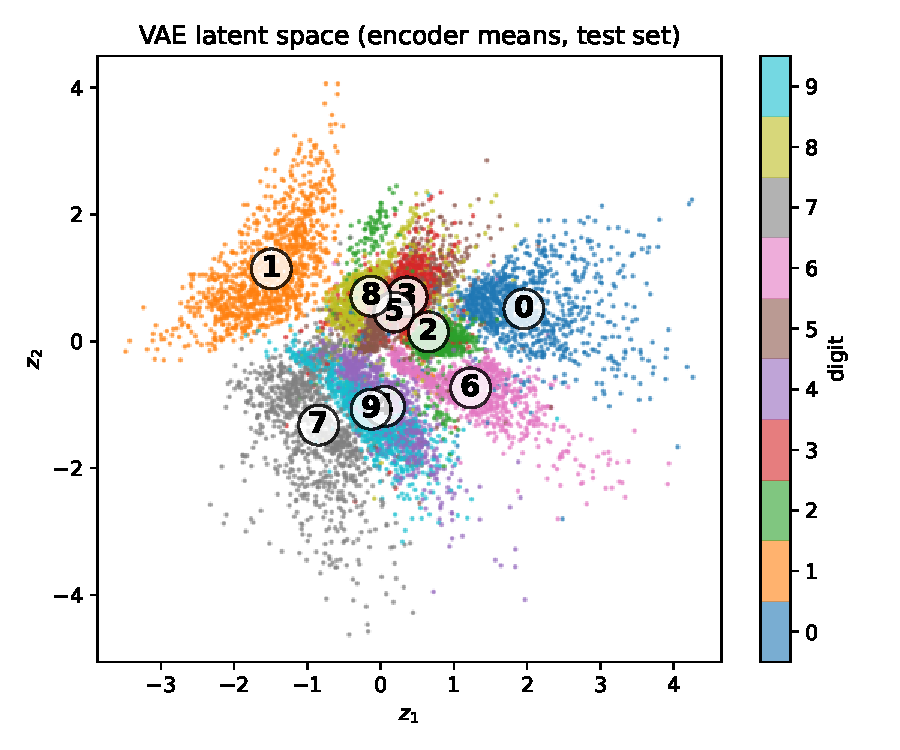
\includegraphics[width=\textwidth,height=0.82\textheight,keepaspectratio]{vae_latent_scatter.pdf}
\end{center}
\caption{The latent space of the VAE: a random subset of the data
  points mapped to their means $\boldsymbol{\mu}$ and coloured by
  their label. This should be compared with Fig.~\ref{fig:latent}, and
  when comparing them look at the scale on the axes; the VAE latent
  space is compact, centred on the origin and has no gaps between the
  clusters.\label{fig:vae_latent}}
\end{figure}

\begin{figure}
\begin{center}
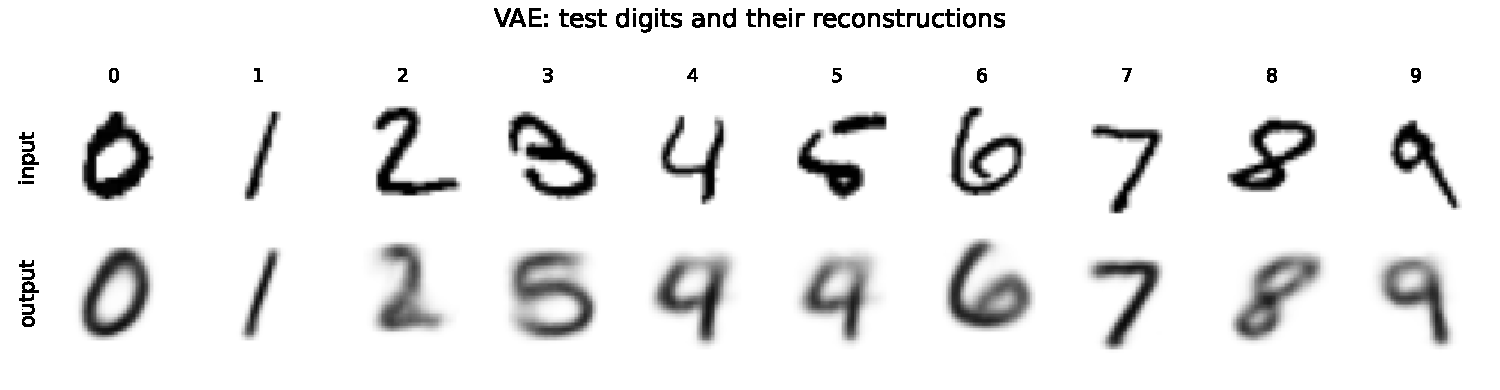
\includegraphics[width=0.95\textwidth]{vae_reconstructions.pdf}
\end{center}
\caption{The VAE reconstruction for an example of each digit, the
  original on top, the reconstruction below. These are a little
  blurrier than the reconstructions in Fig.~\ref{fig:recon}; this is
  the price of the KL term.\label{fig:vae_recon}}
\end{figure}

The latent space is shown in Fig.~\ref{fig:vae_latent} and the
difference from the autoencoder latent space in Fig.~\ref{fig:latent}
is obvious. The autoencoder was free to put the digits wherever it
liked, and what it liked was to send them off in long arms in
different directions with a crowded blob in the middle; the VAE has
been told that the means should be near zero and the standard
deviations near one, and what we get is a compact latent space,
centred on the origin, with the clusters for the different digits
packed up against each other without gaps between them. Again, the
labels are only there in the picture, the learning is unsupervised and
the network was not told which digit was which. There is a cost and it
can be seen in the reconstructions in Fig.~\ref{fig:vae_recon}, which
are a little blurrier than the ones the autoencoder managed. This is
what you would expect: the decoder is no longer being asked to
reconstruct an image from one particular point, it is being asked to
reconstruct it from a noisy cloud of points, and since the clouds for
similar images overlap the best it can do at a given point is
something like an average of all the images that might have been sent
there. The loss is a compromise between the reconstruction error,
which would like the clouds to be small and far apart, and the KL
term, which would like every one of them to be a standard normal
sitting at the origin.

\begin{figure}
\begin{center}
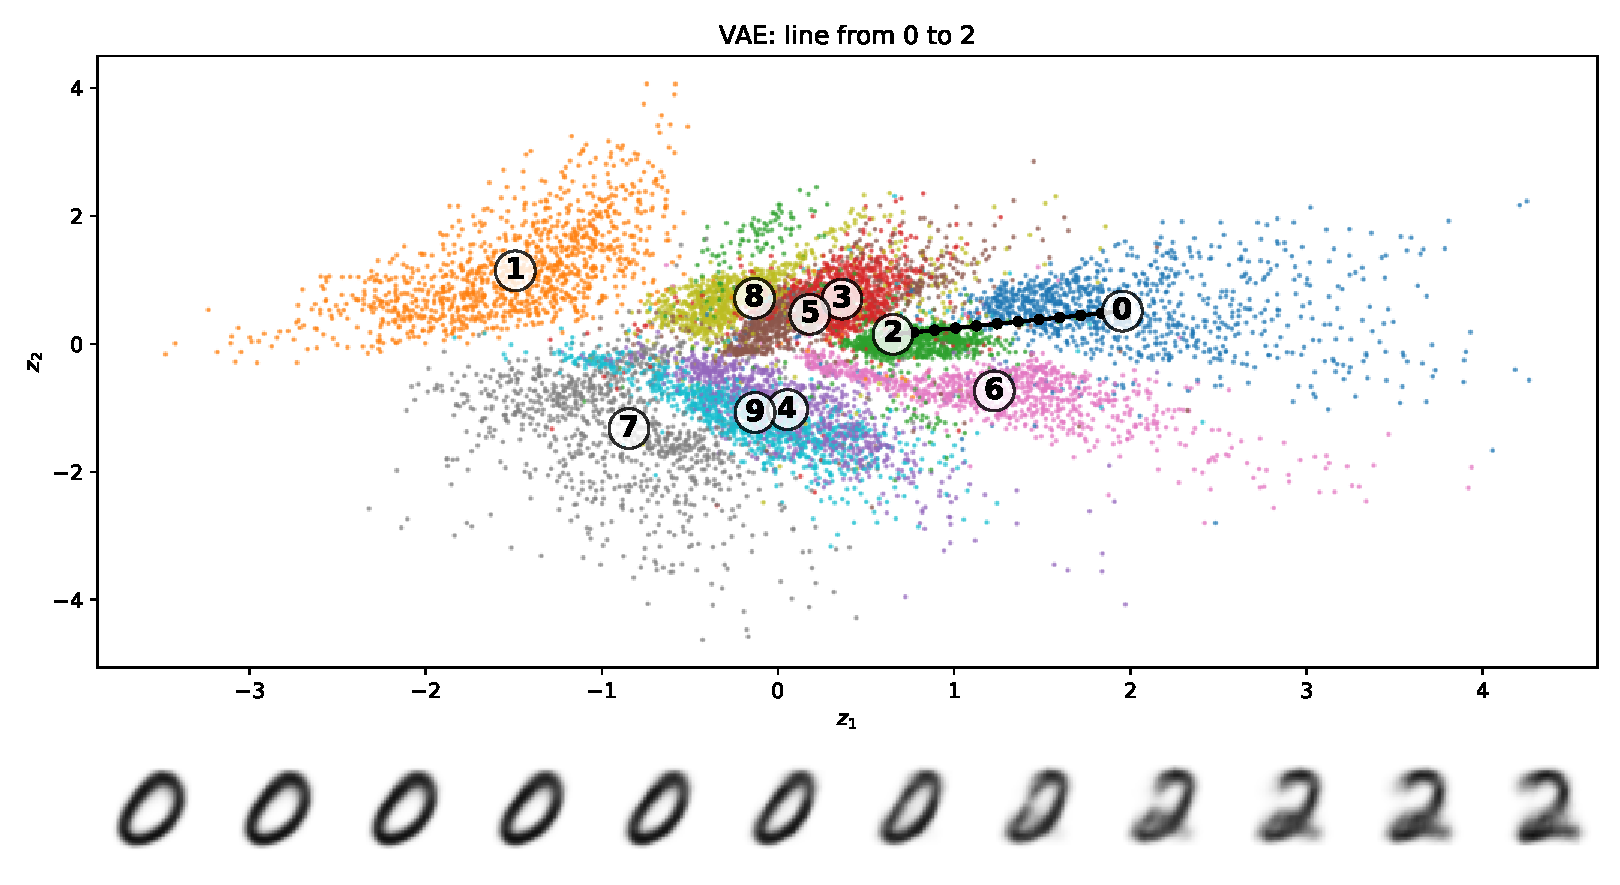
\includegraphics[width=\textwidth,height=0.4\textheight,keepaspectratio]{vae_latent_line_0_2.pdf}

\vskip 0.5cm

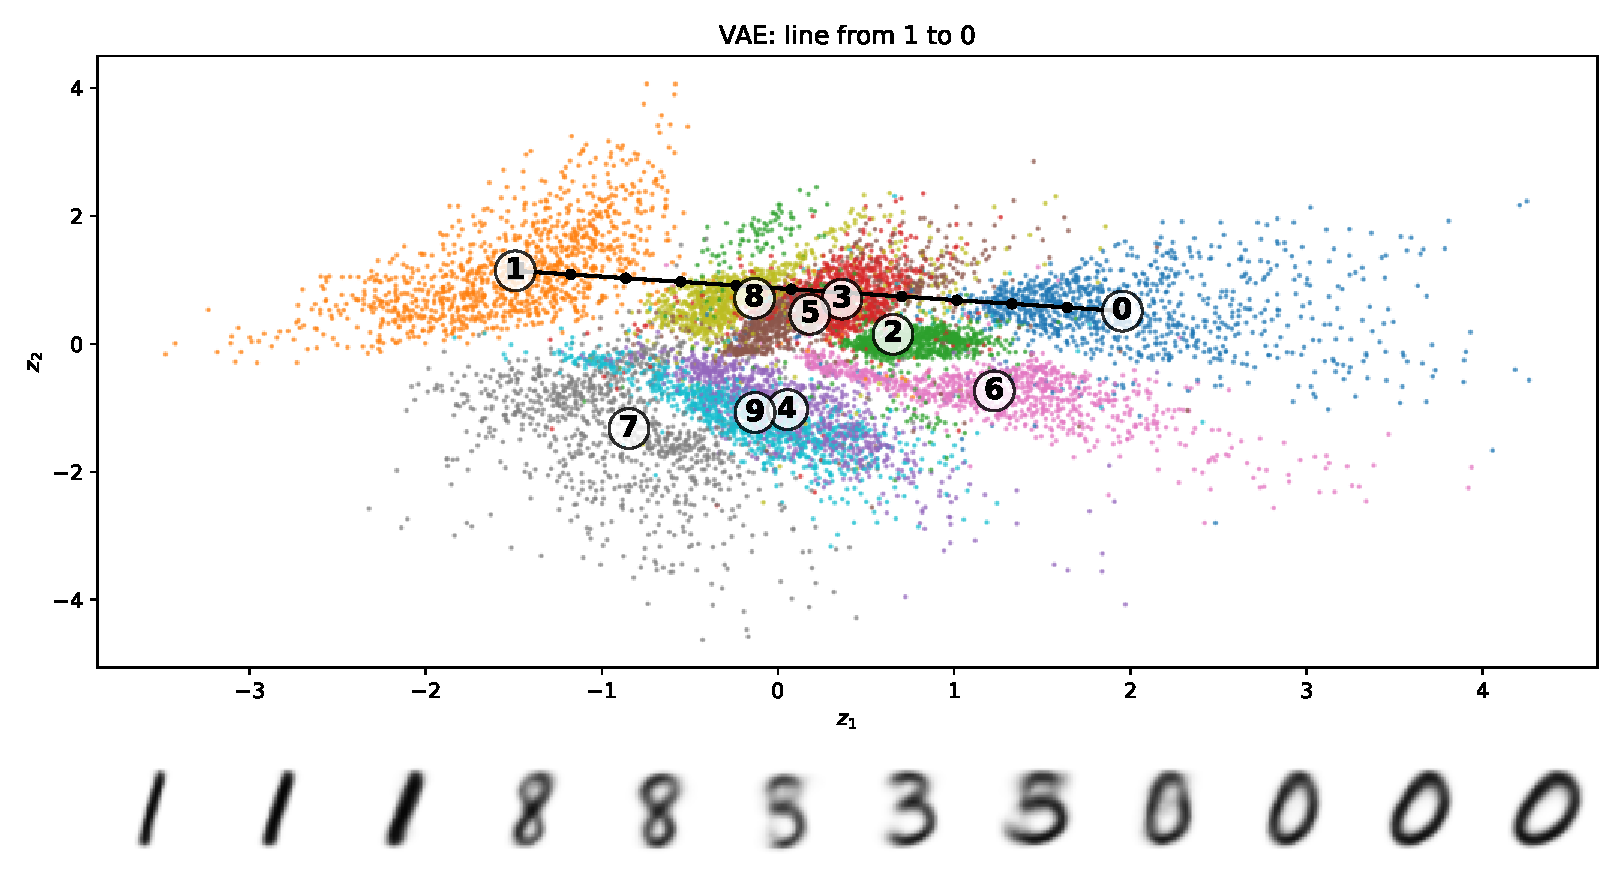
\includegraphics[width=\textwidth,height=0.4\textheight,keepaspectratio]{vae_latent_line_1_0.pdf}
\end{center}
\caption{Two straight lines through the VAE latent space, the first
  from the zeros to the twos, the second from the ones to the zeros,
  with the reconstruction at points along each line. The path between
  clusters now decodes to digits throughout.\label{fig:vae_lines}}
\end{figure}

\begin{figure}
\begin{center}
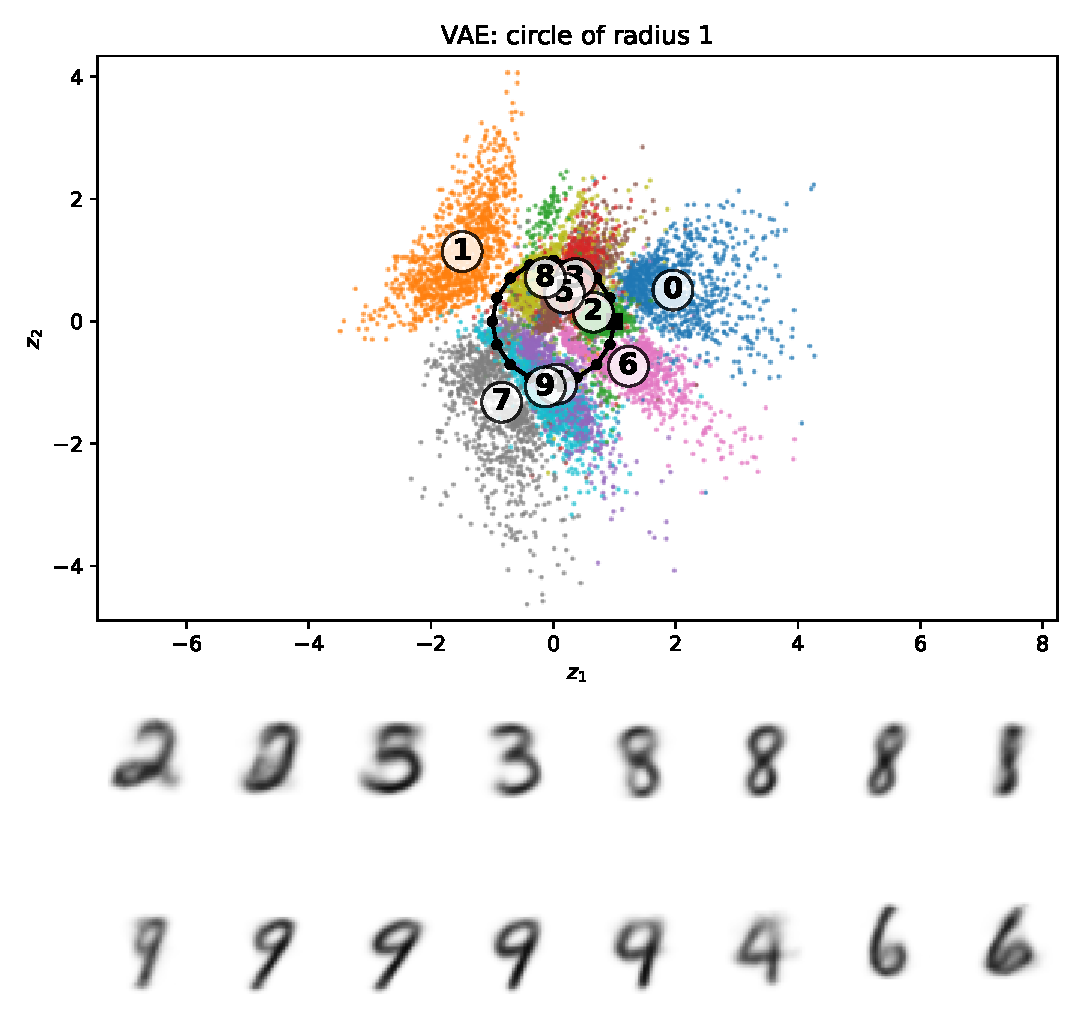
\includegraphics[width=\textwidth,height=0.82\textheight,keepaspectratio]{vae_latent_circle_1.pdf}
\end{center}
\caption{A circle through the VAE latent space, to be compared with
  Fig.~\ref{fig:circle}; again points around the circle are
  reconstructed, showing one digit morphing into another.\label{fig:vae_circle}}
\end{figure}

\begin{figure}
\begin{center}
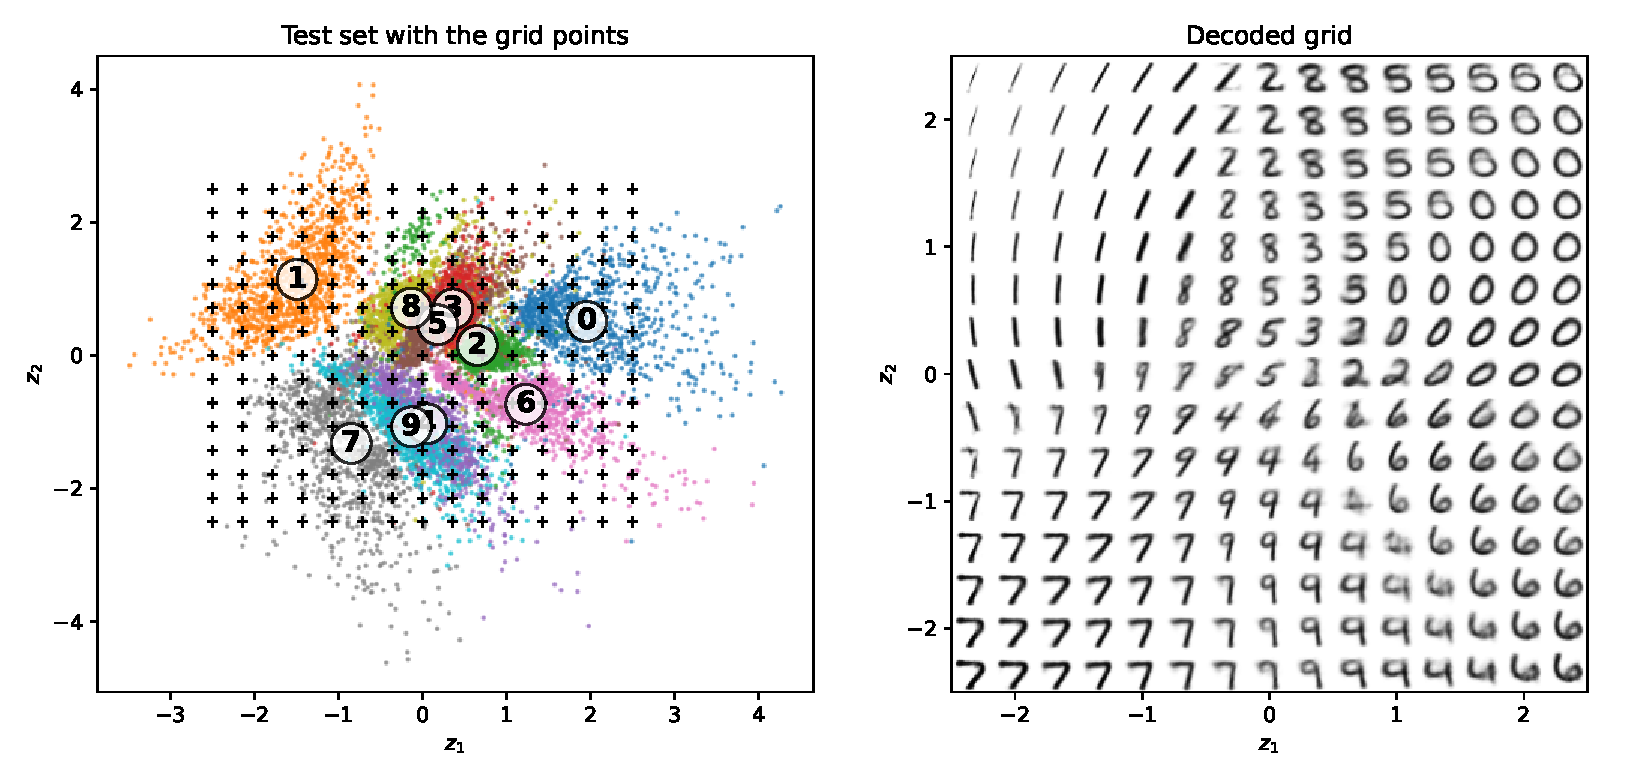
\includegraphics[width=\textwidth,height=0.82\textheight,keepaspectratio]{vae_latent_grid.pdf}
\end{center}
\caption{A grid of points in the VAE latent space and their
  reconstructions, to be compared with Fig.~\ref{fig:grid}.\label{fig:vae_grid}}
\end{figure}

What we have paid for with the blurring is a latent space without
holes, and this is what Fig.~\ref{fig:vae_lines},
Fig.~\ref{fig:vae_circle} and Fig.~\ref{fig:vae_grid} are intended to
show. In Fig.~\ref{fig:vae_lines} we walk in a straight line from one
cluster to another, from the zeros to the twos and from the ones to
the zeros, decoding as we go, and the thing to notice is that the path
decodes to digits throughout; in the autoencoder a journey like this
would cross one of the gaps, where the decoder had never been trained
and the reconstruction did not look like anything. In the same way
Fig.~\ref{fig:vae_circle} and Fig.~\ref{fig:vae_grid} repeat for the
VAE what we did in Fig.~\ref{fig:circle} and Fig.~\ref{fig:grid} for
the autoencoder, and the complaint we made about Fig.~\ref{fig:grid},
that the change from one digit to another did not `stick' to the space
of plausible digits, has largely been answered. It is worth saying
again why this has happened: every training image is decoded from a
slightly different point each time it is presented, so the decoder is
trained on the whole neighbourhood of each image, not just on a single
point, and the KL term has pulled all these neighbourhoods together
around the origin so that they overlap and cover the space.

\begin{figure}
\begin{center}
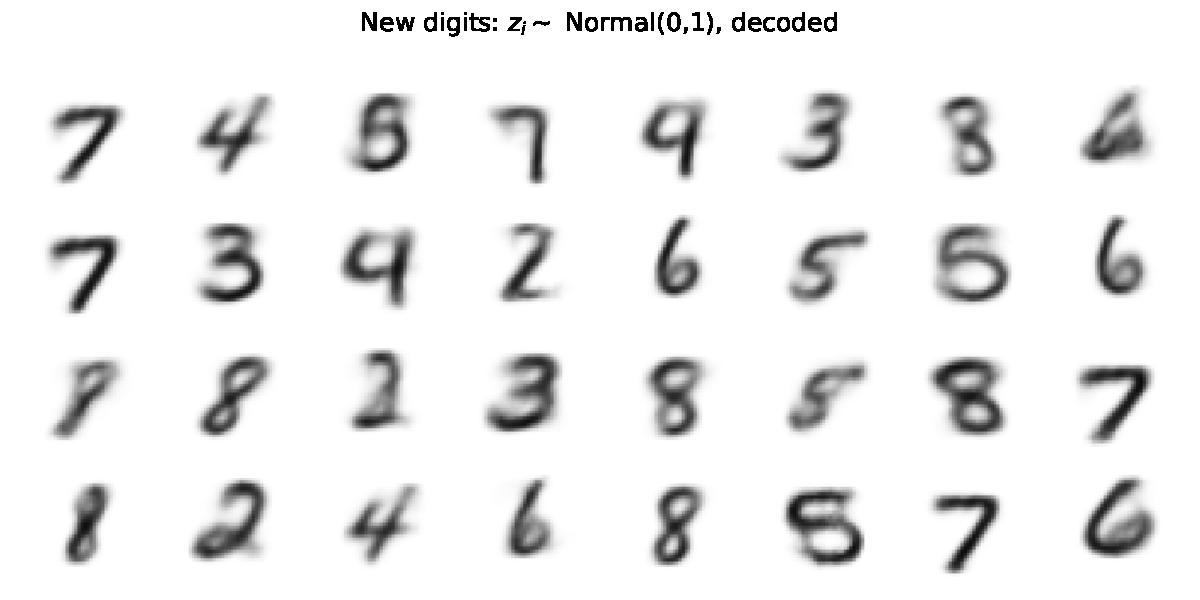
\includegraphics[width=\textwidth,height=0.6\textheight,keepaspectratio]{vae_samples.pdf}
\end{center}
\caption{New digits: each of these was made by sampling
  $z_i\sim\text{Normal}(0,1)$ and applying the decoder, no training
  image was involved.\label{fig:vae_samples}}
\end{figure}

Finally, and this is the point of calling it a generative space, we
can throw away the encoder altogether:
\begin{equation}
  \textcolor{red}{z_i\sim\text{Normal}(0,1)} \rightarrow \hat{\mathbf{x}}=g(\mathbf{z})
\end{equation}
This is just the generative story from the formal description, run
forwards: pick a point from the prior and decode it. Some examples are
shown in Fig.~\ref{fig:vae_samples}; these are new digits, they are
not reconstructions of anything in the dataset, and they look like
digits because the prior we are sampling from is the distribution the
KL term was pushing the encoded data towards during training. Doing
the same thing with the ordinary autoencoder would not work, for one
thing we would not know what distribution to sample from, and for
another, as we saw in Fig.~\ref{fig:grid}, much of the latent space
does not decode to a digit at all.


\end{document}
